
\documentclass{report}

\usepackage[utf8]{inputenc}
\usepackage[italian]{babel}
\usepackage{import}
\usepackage{todonotes}
\usepackage{color}
\usepackage{rotating}
\usepackage[hidelinks]{hyperref}
\usepackage{url}
\usepackage{pdfpages}
\usepackage{siunitx}
\usepackage{pdflscape}
\usepackage{subfig}
\usepackage[euler]{textgreek}
\usepackage{mhchem}

\usepackage{enumerate} 
\usepackage{amsmath}
\usepackage{amsfonts}

\usepackage[signatures,swapnames,sans]{frontespizio}

\usepackage{geometry}
\geometry{portrait, margin=3cm}
\usepackage{siunitx}
\usepackage{booktabs}

\renewcommand*\figurename{Figura}

\newcommand{\sub}[1]{\textsubscript{#1}}
\newcommand{\super}[1]{\textsuperscript{#1}}
\newcommand{\parallelsum}{\mathbin{\!/\mkern-5mu/\!}}

\newcommand{\Fig}[0]{Fig.}

\usepackage{titlesec}

\titleformat{\chapter}{\normalfont\huge}{}{20pt}{\huge\bfseries}

\linespread{1.3}


%% COMANDI UTILI
%\begin{table}[h]
%	\centering
%	\begin{tabular}{|c|c|c|}
%	\cline{2-3} 
%	\multicolumn{1}{c|}{} & \textbf{Valore nominale} & \textbf{Valore misurato}\\ 
%		%\hline
%		%{} & \textbf{Valore nominale} & \textbf{Valore misurato} \\ 
%		\hline
%		$\mathbf{R_1}$ & \SI{18}{k\ohm} & \SI{17.977}{k\ohm} \\ 
%		\hline
%		$\mathbf{R_2}$& \SI{1.8}{k\ohm} & \SI{1.815}{k\ohm} \\ 
%		\hline
%	\end{tabular}
%\caption{Misure delle resistenze utilizzate per il circuito.}
%\label{table:mis_res}
%\end{table}
%\begin{figure}[h!]
%\centering
%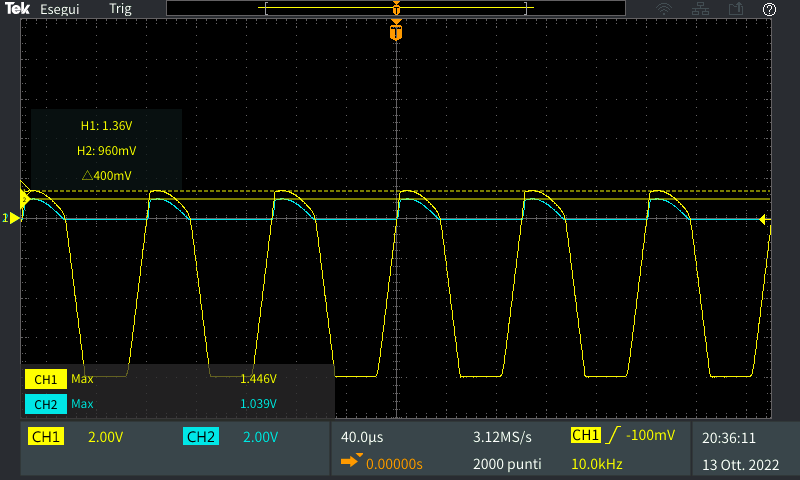
\includegraphics[height=6.5cm]{immagini/TEK00018}\\(a)\\[1ex]
%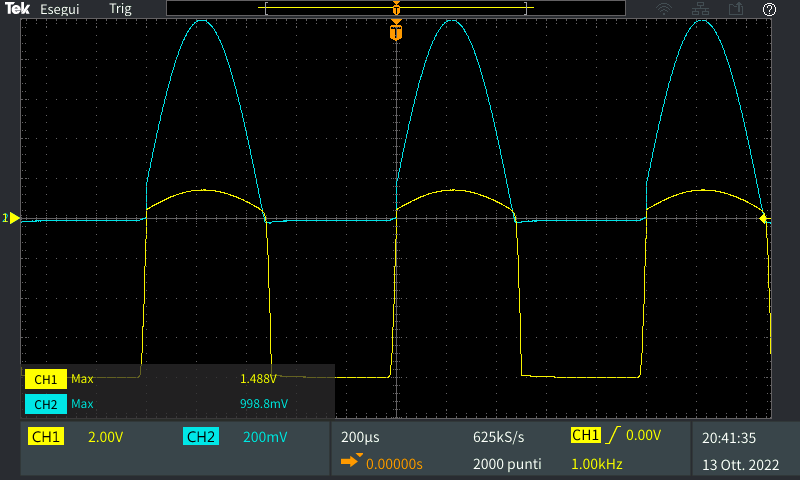
\includegraphics[height=6.5cm]{immagini/TEK00019}\\(b)
%\caption{Risposta del circuito con accoppiamento DC (a) e accoppiamento AC (b).}
%	\label{figura:accopp}
%\end{figure}

\begin{document}
\addtocounter{chapter}{+1}
	\begin{frontespizio}
		\Margini{3cm}{3cm}{3cm}{3cm}
		\Universita{Bergamo}
		\Logo[43.332mm]{unibg-mark}
		\Divisione{Scuola di Ingegneria}
		\Corso[Laurea Magistrale]{Ingegneria Informatica}
		\Titolo{Laboratorio di Elettronica}
		\Sottotitolo{Relazione esperienza di laboratorio 2}
		\Punteggiatura{}
		\NRelatore{Prof.}{Prof.}
		\Relatore{Luigi Gaioni}
		\Candidato[1058231]{Giulia Allievi}
		\Candidato[1059640]{Martina Fanton}
		\Annoaccademico{2022--2023}
		\begin{Preambolo*}
			\usepackage[italian]{babel}
			\usepackage[T1]{fontenc}
			\usepackage[utf8]{inputenc}
			\usepackage{microtype}
			\usepackage{lmodern}
			\graphicspath{{img/}}
			
			\renewcommand{\frontinstitutionfont}{\fontsize{14}{17}\bfseries\scshape}
			\renewcommand{\fronttitlefont}{\fontsize{17}{21}\bfseries\scshape}
			\renewcommand{\frontfootfont}{\fontsize{12}{14}\bfseries\scshape}
		\end{Preambolo*}
	\end{frontespizio}

%----------------------------------------------------------------------------------------
%	PAGINA BIANCA
%----------------------------------------------------------------------------------------
\newpage
\null
\thispagestyle{empty}
\newpage

%----------------------------------------------------------------------------------------
%	INTRO
%----------------------------------------------------------------------------------------
% Ho cambiato la struttura per questa relazione così rimane tutto nominato con il numero 2
\chapter{Relazione attività di laboratorio 2}
\section*{Introduzione}
Nei circuiti realizzati in questa attività di laboratorio utilizzeremo dei diodi, in particolare i diodi 1N4148. Un diodo è un dispositivo non lineare perché la corrente che fluisce al suo interno ha un andamento esponenziale in funzione della tensione applicata ai suoi capi, inoltre non è simmetrico perché la corrente può fluire in un solo verso, ovvero dall'anodo al catodo, e non viceversa.
\begin{figure}[h]
	\centering
	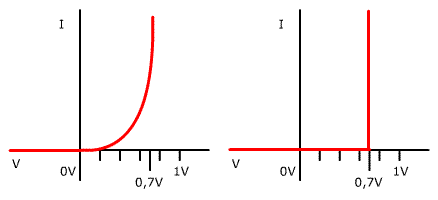
\includegraphics[height=5cm]{immagini/diodo}
	\caption{Caratteristica reale (a destra) e ideale (a destra) di un diodo.}
	\label{figura:diodo}
\end{figure}
\\Nella figura precedente, la figura \ref{figura:diodo} si possono vedere la caratteristica reale ed ideale di un diodo: per studiare più facilemente i circuiti si approssima il comportamento di un diodo e lo si considera spento (OFF) se la tensione applicata ai suoi capi è minore di \SI{0.7}{\volt}; al contrario, se la tensione ai suoi capi è maggiore di questo valore, il diodo è acceso (ON) e lascia fluire la corrente dall'anodo al catodo con una caduta di tensione ai suoi capi di \SI{0.7}{\volt}.
\section{Circuito 1: raddrizzatore passivo a semionda}
\subsection{Schema del circuito e Funzione di Trasferimento}Il primo circuito è il raddrizzatore più semplice che si può realizzare. \`E costituito da un diodo e da una resistenza, il segnale viene applicato all'anodo del diodo e l'uscita del circuito è prelevata al catodo del diodo. Il circuito non viene alimentato, perciò abbiamo un raddrizzatore passivo. \par
\begin{figure}[h]
	\centering
	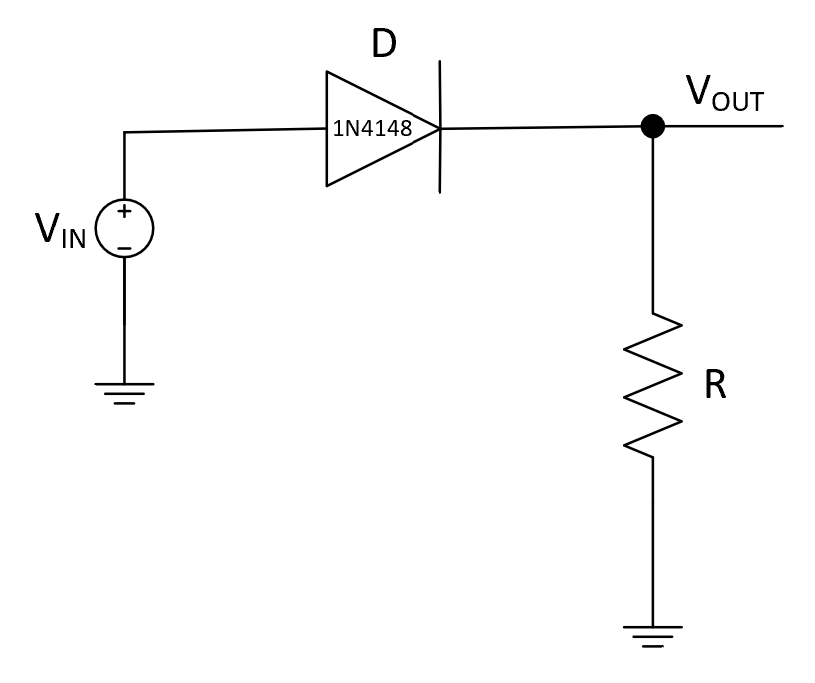
\includegraphics[height=6.5cm]{immagini/schema1}
	\caption{Schema del raddrizzatore passivo a semionda.}
	\label{figura:schema1}
\end{figure}
\noindent La funzione di trasferimento di questo raddrizzatore è:
\begin{equation}
   \begin{cases}
   V_{in}< \SI{0.7}{\volt}\;\;\rightarrow \mathrm{D\;OFF} \Rightarrow V_{out} =\SI{0}{\volt}\\
   V_{in}\ge \SI{0.7}{\volt}\;\;\rightarrow \mathrm{D\;ON}\;\; \Rightarrow V_{out} = V_{in}-\SI{0.7}{\volt}
   \end{cases}
\end{equation}
\subsection{Analisi e dati sperimentali}
% metti che catodo (?) ha una fascia nera
\newpage
\section{Circuito 2: raddrizzatore a semionda di precisione}
\subsection{Schema del circuito e Funzione di Trasferimento}
Modifichiamo il circuito di prima introducendo un'amplificatore operazionale, il \textmu A741. Il diodo si trova ora in reazione all'amplificatore operazionale, nella cosiddetta configurazione a superdiodo: con queste connessioni otteniamo un raddrizzatore di precisione perché eliminiamo la caduta di tensione della giunzione p-n del diodo. Lo svantaggio è che l'OPAMP è un dispositivo attivo, quindi dovremo alimentare il circuito.\par
\begin{figure}[h]
	\centering
	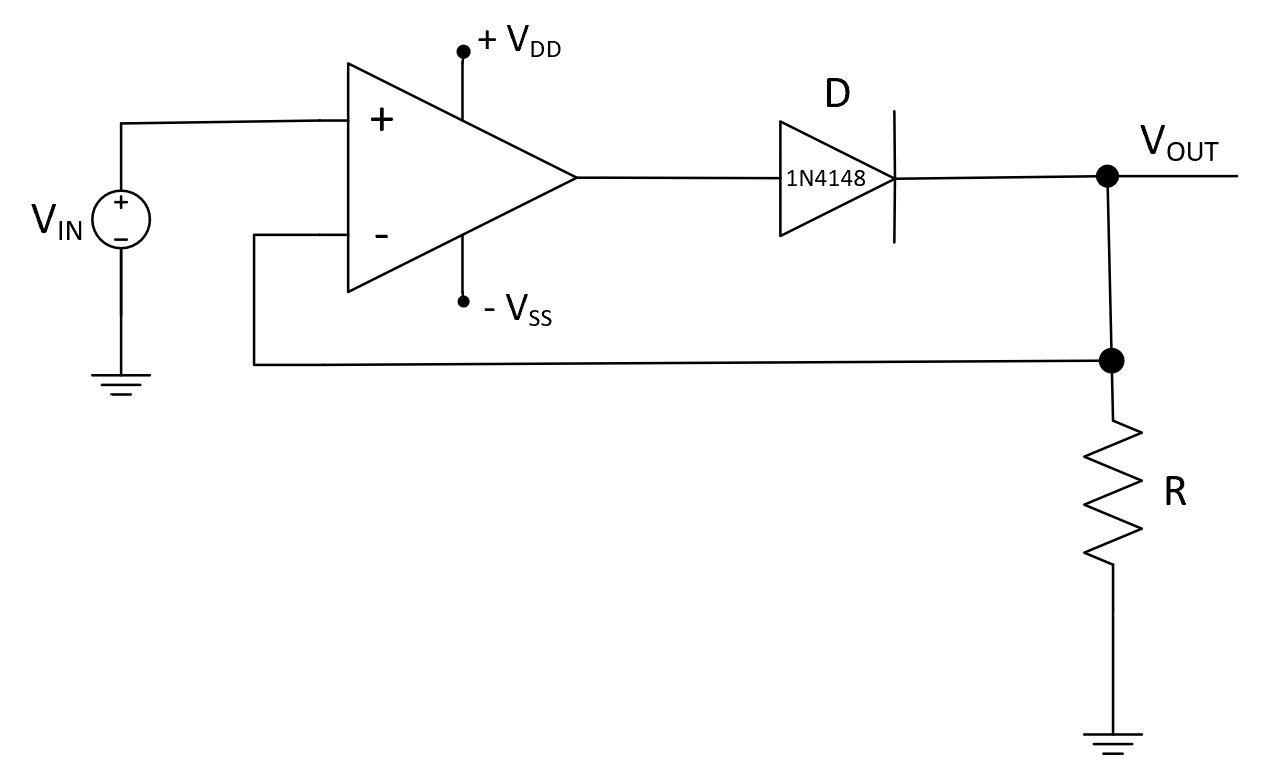
\includegraphics[height=6.5cm]{immagini/schema2}
	\caption{Schema del raddrizzatore a semionda di precisione.}
	\label{figura:schema2}
\end{figure}
\noindent La funzione di trasferimento è:
\begin{equation}
   \begin{cases}
   V_{in}\le \SI{0}{\volt}\;\;\rightarrow \mathrm{D\;OFF} \Rightarrow V_{out} =\SI{0}{\volt}\\
   V_{in}> \SI{0}{\volt}\;\;\rightarrow \mathrm{D\;ON}\;\; \Rightarrow V_{out} = V_{in}
   \end{cases}
\end{equation}
\subsection{Analisi e dati sperimentali}

\newpage
\section{Circuito 3: raddrizzatore a doppia semionda}
\subsection{Schema del circuito e Funzione di Trasferimento}
In questo circuito (come mostrato nella figura \ref{figura:schema3}), a differenza dei precedenti due, sono presenti due diodi: il primo è collegato con l'anodo all'uscita dell'OPAMP e con il catodo al noto $\displaystyle\mathrm{V_{out}}$, mentre il secondo è posizionato nella retroazione del circuito, con l'anodo collegato al nodo $\displaystyle\mathrm{V_{in}}$ e il catodo a $\displaystyle\mathrm{V_{out}}$.\par
La differenza principale di questo circuito rispetto ai precedenti è che non raddrizza solo le semionde negative o positive, ma entrambe, per questo il raddrizzatore è detto \textit{a doppia semionda}. \par
Inoltre il raddrizzatore a doppia semionda presenta due retroazioni negative e in particolare quella costituita dalla sola resistenza R è sempre chiusa permettendo al circuito in esame di non operare in anello aperto.\par % DA CONTROLLARE
In aggiunta l'amplificatore si trova in configurazione invertente e per la presenza di resistenze con valori equivalenti presenta un guadagno pari a -1 (di fatto è un buffer invertente, come si vede dalla figura \ref{figura:}). % Da mettere? (la figura non c'è ancora)
\begin{figure}[h]
	\centering
	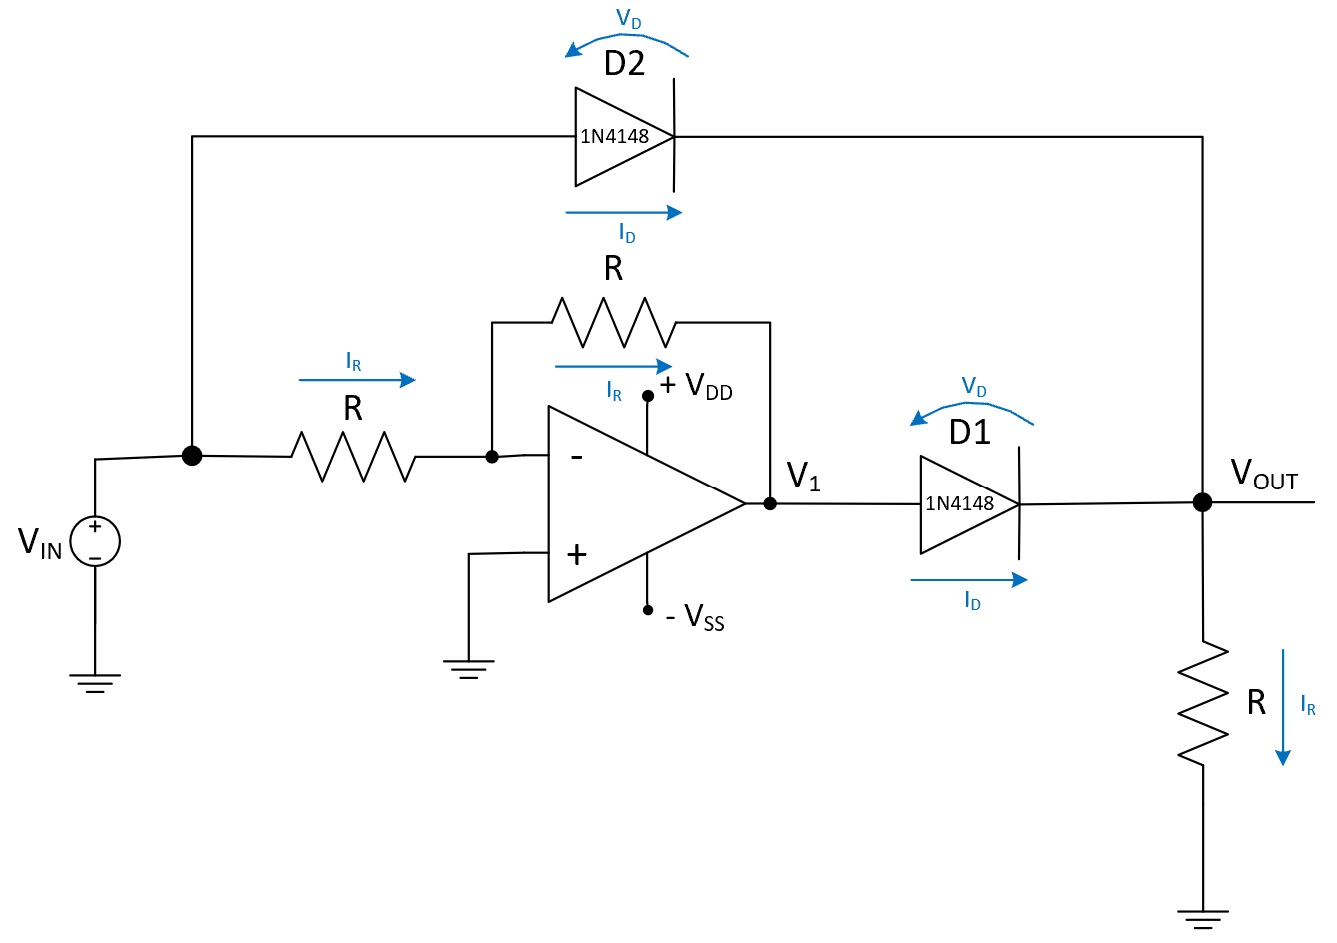
\includegraphics[height=6.5cm]{immagini/schema3}
	\caption{Schema del raddrizzatore a doppia semionda.}
	\label{figura:schema3}
\end{figure}
\\La funzione di trasferimento corrispondente a questo circuito è:

\begin{equation}
   \begin{cases}
   V_{in}\le \SI{-0.7}{\volt}\;\;\indent\indent\rightarrow \mathrm{D_1\; ON, D_2\;OFF}\;\; \Rightarrow V_{out} = -V_{in}-\SI{0.7}{\volt}\\
  \SI{-0.7}{\volt} < V_{in}< \SI{0.7}{\volt}\rightarrow \mathrm{D_1\; OFF, D_2\;OFF} \Rightarrow V_{out} = \SI{0}{\volt}\\
   V_{in}\ge \SI{0.7}{\volt}\;\;\;\;\;\indent\indent\rightarrow \mathrm{D_1\; OFF, D_2\;ON}\;\; \Rightarrow V_{out} = V_{in}-\SI{0.7}{\volt}
   \end{cases}
\end{equation}

\subsection{Analisi e dati sperimentali}
Come primo passo per la costruzione del circuito, sono stati misurati i valori dei componenti che verranno utilizzati. In particolare abbiamo scelto tre resistenze da \SI{12}{k\ohm}. Le loro misure sono state riportate nella tabella \ref{table:mis_res3}.
\begin{table}[h]
	\centering
	\begin{tabular}{|c|c|c|}
		\cline{2-3} 
		\multicolumn{1}{c|}{} & \textbf{Valore nominale} & \textbf{Valore misurato}\\ 
		\hline
		$\mathbf{R_1}$ & \SI{12}{k\ohm} & \SI{11.802}{k\ohm} \\ 
		\hline
		$\mathbf{R_2}$ & \SI{12}{k\ohm} & \SI{11.947}{k\ohm} \\ 
		\hline
		$\mathbf{R_3}$ & \SI{12}{k\ohm} & \SI{11.885}{k\ohm} \\ 
		\hline
	\end{tabular}
	\caption{Misure delle resistenze utilizzate per il circuito.}
	\label{table:mis_res3}
\end{table}
\\Una volta realizzato il circuito sulla breadboard, sono poi state effettuate delle misure (presenti nella tabella \ref{table:misure3}) dei valori di tensione nei vari nodi del circuito considerando i segnali in ingresso e in uscita a diverse frequenze (quelle considerate sono state: \SI{1}{k\hertz}, \SI{10}{k\hertz}, \SI{100}{k\hertz} e \SI{400}{k\hertz}).
\begin{table}[h!]
	\centering
	\begin{tabular}{|c|c|c|c|}
		\hline
		\textbf{Frequenza} & \boldmath$\displaystyle\mathrm{V_{PP,in}}$\textbf{ [V]} & \boldmath$\displaystyle\mathrm{{V_{PP,out}}}$\textbf{ [V]} & \boldmath$\Delta$\textbf{V [V]}\\
		\hline
		1 kHz & 0.980 & 0.520 & 0.460\\
		\hline
		10 kHz & 0.960 & 0.520 & 0.440\\
		\hline
		100 kHz & 0.980 & 0.520 & 0.460\\
		\hline
		400 kHz & 0.528 & 0.288 & 0.240\\
		\hline\end{tabular}
	\caption{Grandezze misurate ad ogni frequenza.}
	\label{table:misure3}
\end{table}
\\Per quanto riguarda la frequenza di \SI{1}{k\hertz}, come si può notare dalla figura \ref{figura:TEK00022}, i segnali presentano un andamento quasi ideale. A questa frequenza si può anche notare la presenza di un offset tra la tensione in ingresso e quella in uscita, che risulta pari a \SI{0.460}{\volt}.
\begin{figure}[h!]
	\centering
	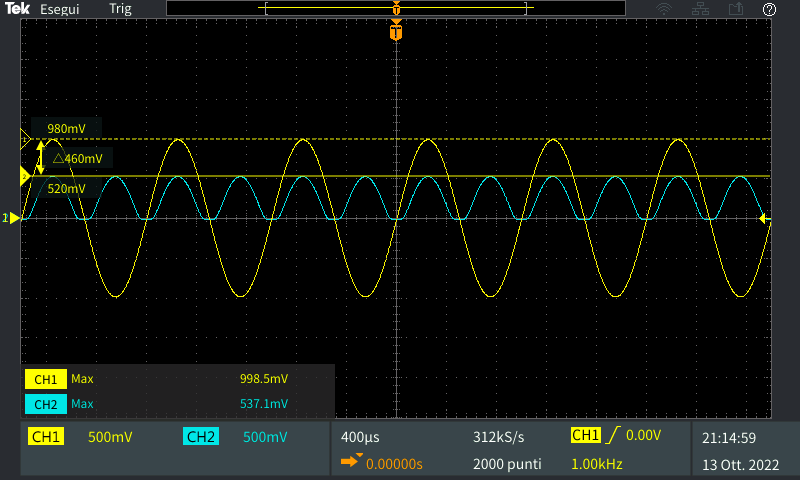
\includegraphics[height=6cm]{immagini/TEK00022}
	\caption{Segnali di $\mathrm{V_1}$ e di $\mathrm{V_{out}}$ con frequenza di \SI{1}{k\hertz}.}
	\label{figura:TEK00022}
\end{figure}
\\Invece se ad esempio si considera la frequenza di \SI{100}{k\hertz}, come si può notare dalla figura \ref{figura:TEK00025}, si vede che i segnali presentano una curva più estesa nella fase di spegnimento del diodo rispetto a quella della fase di accensione. Questo andamento risulta ancora più accentuato nella figura \ref{figura:TEK00030} in cui la frequenza considerata è di \SI{400}{k\hertz}. A questa frequenza vediamo anche che scompaiono le semionde negative, perché non vengono più raddrizzate.
\\Per frequenze maggiori, non ha senso studiare il circuito perché sappiamo che la banda di funzionamento del nostro OPAMP è limitata a circa \SI{100}{k\hertz} e anche la velocità di risposta dei diodi è stata superata.
\begin{figure}[h!]
	\centering
	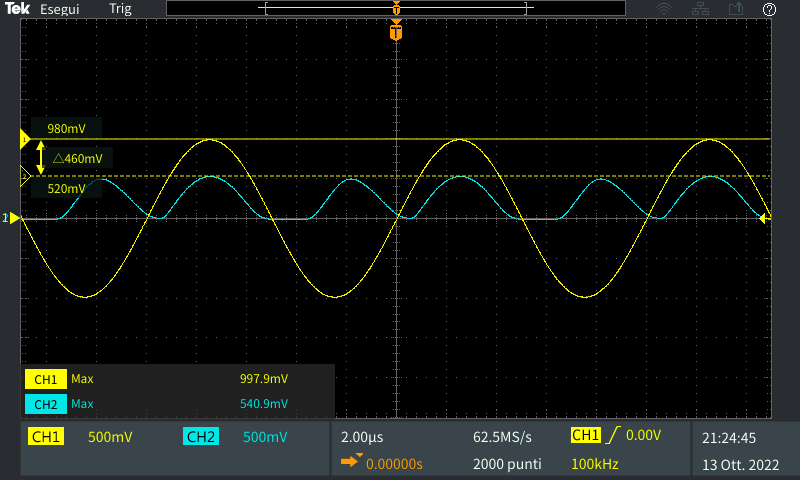
\includegraphics[height=6cm]{immagini/TEK00025}
	\caption{Segnali di $\mathrm{V_1}$ e di $\mathrm{V_{out}}$ con frequenza di \SI{100}{k\hertz}.}
	\label{figura:TEK00025}
\end{figure} 
\begin{figure}[h!]
	\centering
	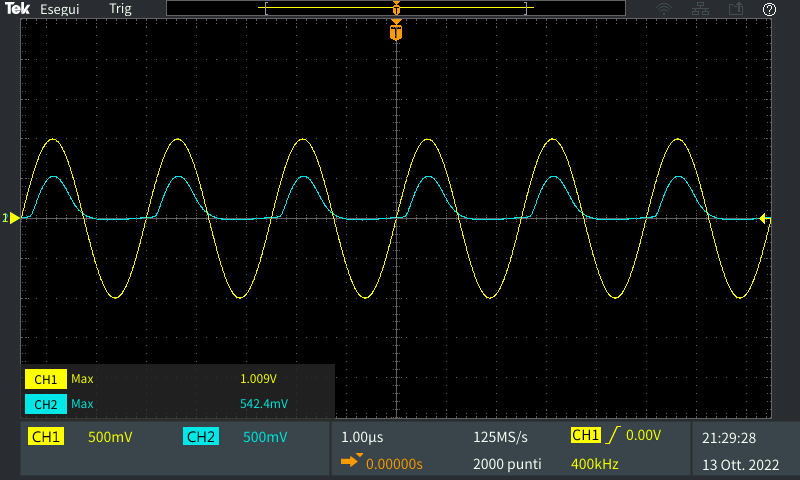
\includegraphics[height=6cm]{immagini/TEK00030}
	\caption{Segnali di $\mathrm{V_1}$ e di $\mathrm{V_{out}}$ con frequenza di \SI{400}{k\hertz}.}
	\label{figura:TEK00030}
\end{figure} 
\\Come si può notare dai grafici di questo circuito, il raddrizzatore a doppia semionda risolve il problema causato dallo swing della tensione $\displaystyle\mathrm{V_1}$ del secondo raddrizzatore analizzato. In questo modo la tensione in uscita all'OPAMP evita di raggiungere i valori delle alimentazioni dell'amplificatore stesso e di determinare proprio degli swing in tensione, che hanno l'effetto di rendere il circuito più lento.\par 
Permane però la caduta di tensione data dalla giunzione p-n dei diodi, perciò il segnale in uscita è leggermente attenuato. Questo può essere critico se il segnale da raddrizzare ha una piccola ampiezza.

%----------------------------------------------------------------------------------------

\end{document}
